% !TEX encoding = UTF-8 Unicode
\documentclass[a4paper, 9pt]{report}

\usepackage[dvipsnames]{xcolor}


\usepackage{amsmath}
\usepackage{amsthm}
\usepackage{amssymb}
\usepackage{dsfont} 



\usepackage{tikz}
\usetikzlibrary{tikzmark}
\usepackage{tcolorbox}


\newcommand{\highlight}[2]{\colorbox{#1!17}{$\displaystyle #2$}}
\DeclareMathOperator*{\argmin}{arg\,min}
\DeclareMathOperator{\MSE}{MSE}
\DeclareMathOperator{\Bias}{Bias}
\DeclareMathOperator{\smCE}{smCE}
\DeclareMathOperator{\dCE}{\mathrm{dCE}}
\DeclareMathOperator{\pGap}{\mathrm{pGap}}
\DeclareMathOperator{\dual}{\mathrm{dual}}
\DeclareMathOperator{\sign}{sign}
\newcommand{\probability}[1]{\mathbb{P}\left(\displaystyle #1 \right)}
\newcommand{\variance}[1]{\mathbb{V}\left[\displaystyle #1 \right]}
\newcommand{\expectation}[2][]{\underset{#1}{\mathbb{E}}\left[\displaystyle #2 \right]}
\newcommand{\Trace}[1]{\mathrm{Tr}\left[\displaystyle #1 \right]}


\begin{document}


\begin{equation*}
	R_X(\beta^*, \beta) = \tikzmarknode{Bias}{\highlight{blue}{\left\|\expectation{\beta^*|X}-\beta\right\|^2_\Sigma}} + \tikzmarknode{Variance}{\highlight{red}{\Trace{\variance{\beta^*|X}\Sigma}}}
\end{equation*}

\begin{tikzpicture}[overlay, remember picture, >=stealth, nodes={align=left, inner ysep=1pt}, <-]
	% Pour Bias
	\path (Bias.south) ++ (0, +3.5em) node[anchor=south east, color=blue!60] (Bias_point) {$\displaystyle B_X(\beta^*, \beta)$};
	\draw [color=blue!80] (Bias.north) |- ([xshift=-0.3ex, color=blue] Bias_point.south west);
	
	% Pour Variance
	\path (Variance.north) ++ (0em, -2.5em) node[anchor=north west, color=red!60] (Variance_point) {$\displaystyle V_X(\beta^*, \beta)$};
	\draw [color=red!80] (Variance.south) |- ([xshift=-0.3ex, color=red] Variance_point.north east);
\end{tikzpicture}\newline\newline





\begin{equation*}
	f(x) = \frac{1}{\displaystyle 1+e^{\displaystyle-(x_1w_1 + \ldots + x_dw_d)}} = \frac{1}{\displaystyle 1+e^{\displaystyle-\langle x, \tikzmarknode{RLweight}{\highlight{red}{w}}\rangle}}
\end{equation*}

\begin{tikzpicture}[overlay, remember picture, >=stealth, nodes={align=left, inner ysep=1pt}, <-]
	\path (RLweight.north) ++ (0em, -2em) node[anchor=north west, color=red!60] (RLweight_point) {$w = (w_1, \ldots, w_d)\in \mathbb{R}^d$};
	\draw [color=red!80] (RLweight.south) |- ([xshift=-0.3ex, color=red] RLweight_point.north east);
\end{tikzpicture}





\begin{figure}
	\centering
	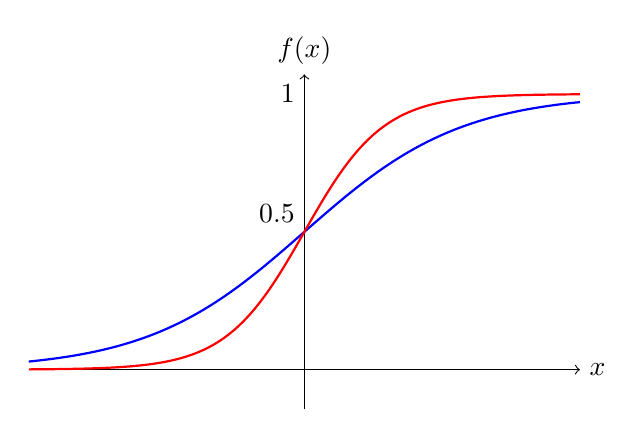
\begin{tikzpicture}[scale=1, samples=200, domain=-3.5:3.5]
		\draw[->] (-3.5, 0) -- (3.5, 0) node[right]{$x$};
		\draw[->] (0, -0.5) -- (0, 3.75) node[above]{$f(x)$};
		\draw (0, 3.5) node[left]{$1$};
		\draw (0, 1.75) node[above left]{$0.5$};
		\draw[color=blue, thick] plot(\x, {3.5/(1+exp(-\x))});
		\draw[color=red, thick] plot(\x, {3.5/(1+exp(-2*\x))});
	\end{tikzpicture}
	\caption{${\color{blue}\displaystyle f(x)=\frac{1}{1+e^{-x}}}$ et ${\color{red}\displaystyle f(x)=\frac{1}{1+e^{-2x}}}$}
\end{figure}


\begin{figure}
	\centering
	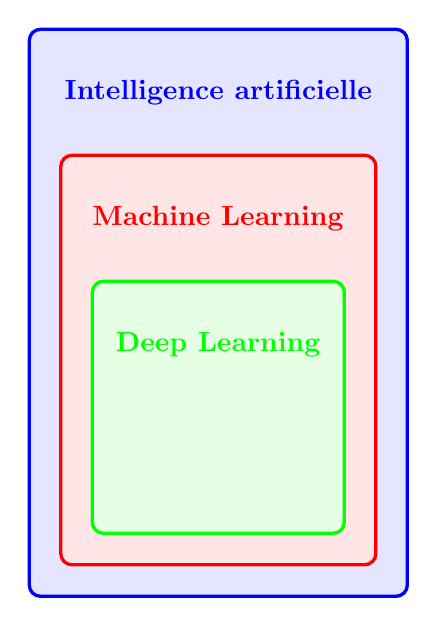
\begin{tikzpicture}[scale=0.8]
		\draw[blue, very thick, rounded corners, fill=blue!10] (0, 0) rectangle (6, 9);
		\draw[red, very thick, rounded corners, fill=red!10] (0.5, 0.5) rectangle (5.5, 7);
		\draw[green, very thick, rounded corners, fill=green!10] (1, 1) rectangle (5, 5);
		\draw (3, 8) node[blue]{\textbf{Intelligence artificielle}};
		\draw (3, 6) node[red]{\textbf{Machine Learning}};
		\draw (3, 4) node[green]{\textbf{Deep Learning}};
	\end{tikzpicture}
\end{figure}



\begin{figure}
	\centering
	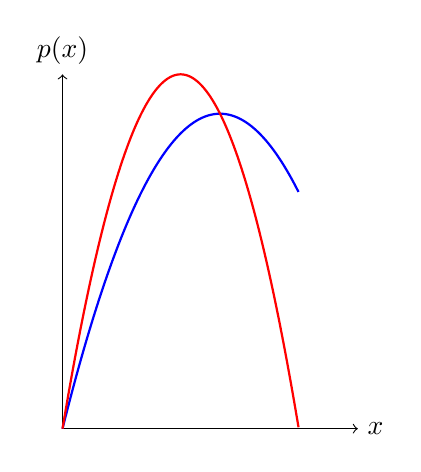
\begin{tikzpicture}[scale=3, samples=200, domain=0:1]
		\draw[->] (0, 0) -- (1.25, 0) node[right]{$x$};
		\draw[->] (0, 0) -- (0, 1.5) node[above]{$p(x)$};
		\draw[color=blue, thick] plot(\x, {-3*\x*\x+4*\x});
		\draw[color=red, thick] plot(\x, {-6*\x*\x+6*\x});
	\end{tikzpicture}
	\caption{Comparaison de deux distributions}
\end{figure}


\begin{figure}
	\centering
	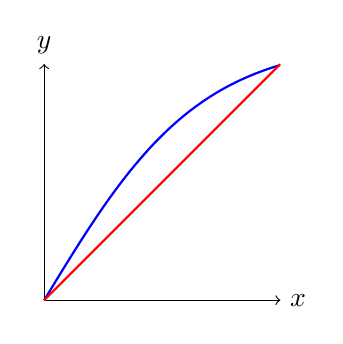
\begin{tikzpicture}[scale=3, samples=200, domain=0:1]
		\draw[->] (0, 0) -- (1, 0) node[right]{$x$};
		\draw[->] (0, 0) -- (0, 1) node[above]{$y$};
		\draw[color=blue, thick] plot(\x, {1.1*tanh(1.5*\x});
		\draw[color=red, thick] plot(\x, {\x});
	\end{tikzpicture}
	\caption{Comparaison de deux liens différents entre $x$ et $y$}
\end{figure}


\end{document}